\documentclass{../../oss-apphys}

\begin{document}
\genheader

\gentitle{2}{FLUID MECHANICS \& THERMODYNAMICS}{19 \& 20}

\genmultidirections

\gengravity

\raggedcolumns
\begin{multicols}{2}

  \begin{enumerate}[leftmargin=18pt]

  \item Two blocks of different sizes and masses float in a tray of water. Each
    block is half submerged, as shown in the figure. Water has a density of
    \SI{1000}{\kilo\gram\per\metre^3}. What can be concluded about the
    densities of the two blocks?
    
    \pic{.39}{mc-q1.png}
    \begin{enumerate}[noitemsep,topsep=0pt,leftmargin=18pt,label=(\Alph*)]
    \item\vspace{-.1in} The two blocks have different densities, both of which
      are less than \SI{1000}{kg/m^3}.
    \item The two blocks have the same density of \SI{500}{kg/m^3}.
    \item The two blocks have the same density, but the density cannot be
      determined with the information given.
    \item The larger block has a greater density than the smaller block, but
      the densities of the blocks cannot be determined with the information
      given.
    \end{enumerate}

  \item The figure shows four cylinders of various diameters filled to different
    heights with water. A hole in the side of each cylinder is plugged by a
    cork. All cylinders are open at the top. The corks are removed. Which
    of the following is the correct ranking of the velocity of the water ($v$)
    as it exits each cylinder?
    
    \pic{.4}{mc-q2.png}
    \begin{enumerate}[noitemsep,topsep=0pt,leftmargin=18pt,label=(\Alph*)]
    \item $v_A > v_D > v_C > v_B$
    \item $v_A = v_D > v_C > v_B$
    \item $v_B > v_C > v_A = v_D$
    \item $v_C > v_A = v_B = v_D$
    \end{enumerate}
  \end{enumerate}
  
  \textbf{Questions 3 and 4}

  Four differently shaped sealed containers are completely filled with alcohol,
  as shown in the figure. Containers A and B are cylindrical. Containers C and
  D are truncated conical shapes. The top and bottom diameters of the
  containers are shown.
  \pic{.45}{mc-q3-4.png}
  \begin{enumerate}[leftmargin=18pt,start=3]
    
  \item Which of the following is the correct ranking of the pressure ($P$) at
    the bottom of the containers?
    \begin{enumerate}[noitemsep,topsep=0pt,leftmargin=18pt,label=(\Alph*)]
    \item $P_A = P_B = P_C = P_D$
    \item $P_A = P_D > P_C = P_B$
    \item $P_A > P_D > P_C > P_B$
    \item $P_D > P_A > P_C > P_B$
    \end{enumerate}

  \item The force on the bottom of container A due to the fluid inside the
    container is F. What is the force on the bottom of container B due to
    the fluid inside?
    \begin{enumerate}[noitemsep,topsep=0pt,leftmargin=18pt,label=(\Alph*)]
    \item $F$
    \item $F/4$
    \item $F/8$
    \item $F/16$
    \end{enumerate}

    \columnbreak
    
  \item Two cylinders filled with a fluid are connected by a pipe so that fluid
    can pass between the cylinders, as shown in the figure. The cylinder
    on the right has 4 times the diameter of the cylinder on the left. Both
    cylinders are fitted with a movable piston and a platform on top. A
    person stands on the left platform. Which of the following lists the
    correct number of people that need to stand on the right platform so
    neither platform moves. Assume that the platform and piston have
    negligible mass and that all the people have the same mass.

    \vspace{-.1in}\pic{.35}{mc-q5.png}
    \begin{enumerate}[noitemsep,topsep=0pt,leftmargin=18pt,label=(\Alph*)]
    \item \num{16} people
    \item \num{4} people
    \item \num{1} person
    \item It is impossible to balance the system because you need 1/16 of a
      person on the right side.
    \end{enumerate}

  \item A mass ($m$) is suspended in a fluid of density ($\rho$) by a string,
    as shown in the figure below. The tension in the string is $T$. Which of
    the following is an appropriate equation for the buoyancy force? Select
    two answers.
    \begin{center}
      \vspace{-.15in}\pic{.3}{mc-q6.png}
    \end{center}
    \begin{enumerate}[noitemsep,topsep=0pt,leftmargin=18pt,label=(\Alph*)]
    \item $F_b=mg$
    \item $F_b=mg-T$
    \item $F_c=a_2 \rho gh_1$
    \item $F_d=a\rho g(h-h_2)$
    \end{enumerate}
    
  \item Three wooden blocks of different masses and sizes float in a container
    of water, as shown in the figure. Each of the masses has a weight on top.
    Which of the following correctly ranks the buoyancy force on the wooden
    blocks?
    \begin{center}
      \vspace{-.15in}\pic{.35}{mc-q7.png}
    \end{center}
    \begin{enumerate}[noitemsep,topsep=0pt,leftmargin=18pt,label=(\Alph*)]
    \item $A > B = C$
    \item $A = B > C$
    \item $B > A = C$
    \item $B > A > C$
    \end{enumerate}
    
  \item Two blocks of the same dimensions are floating in a container of water,
    as shown in the figure. Which of the following is a correct statement about
    the two blocks?
    \begin{center}
      \vspace{-.15in}\pic{.35}{mc-q8.png}
    \end{center}
    \begin{enumerate}[noitemsep,topsep=0pt,leftmargin=18pt,label=(\Alph*)]
    \item The net force on both blocks is the same.
    \item The buoyancy force exerted on both blocks is the same.
    \item The density of both blocks is the same.
    \item The pressure exerted on the bottom of each block is the same.
    \end{enumerate}

    \columnbreak
    
  \item The figure shows four cubes of the same volume at rest in a container
    of water. Cube C is partially submerged. Cubes A, B, and D are fully
    submerged, with B resting on the bottom of the container. Which of the
    following correctly ranks the densities ($\rho$) of the cubes? Assume the
    water to be incompressible.
    \begin{center}
      \vspace{-.15in}
      \pic{.3}{mc-q9.png}
    \end{center}
    \begin{enumerate}[noitemsep,topsep=0pt,leftmargin=18pt,label=(\Alph*)]
    \item $\rho_C >\rho_D >\rho_A >\rho_B$
    \item $\rho_B >\rho_A >\rho_D >\rho_C$
    \item $\rho_B >\rho_A =\rho_D >\rho_C$
    \item $\rho_B >\rho_A =\rho_D =\rho_C$
    \end{enumerate}

  \item A beaker of water sits on a balance. A metal block with a mass of
    \SI{70}{\gram} is held suspended in the water by a spring scale in position
    1, as shown in the figure. In this position, the reading on the balance is
    \SI{1260}{\gram}, and the spring scale reads \SI{120}{g}. When the block is
    lifted from the water to position 2, what are the readings on the balance
    and spring scale?
    \begin{center}
      \vspace{-.15in}
      \pic{.2}{mc-q10.png}

      \begin{tabular}{c c c}
        & \textbf{Balance reading} & \textbf{Spring scale reading}\\
        (A) & \SI{1190}{\gram} & \SI{120}{\gram}\\
        (B) & \SI{1190}{\gram} & \SI{190}{\gram}\\
        (C) & \SI{1260}{\gram} & \SI{120}{\gram}\\
        (D) & \SI{1330}{\gram} & \SI{120}{\gram}
      \end{tabular}
    \end{center}

    \columnbreak
    
  \item Blood cells pass through an artery that has a buildup of plaque along
    both walls, as shown in the figure. Which of the following correctly
    describes the behavior of the blood cells as they move from the right
    side of the figure through the area of plaque? Assume the blood cells
    can change volume.
    \begin{center}
      \vspace{-.15in}
      \pic{.25}{mc-q11.png}
     \end{center}
    \begin{enumerate}[noitemsep,topsep=0pt,leftmargin=18pt,label=(\Alph*)]
    \item\vspace{-.1in} The blood cells increase in speed and expand in volume.
    \item The blood cells increase in speed and decrease in volume.
    \item The blood cells decrease in speed and expand in volume.
    \item The blood cells decrease in speed and decrease in volume.
    \end{enumerate}
    
  \item Firefighters use a hose with a \SI{2}{cm} exit nozzle connected to a
    hydrant with an \SI{8}{cm} diameter opening to attack a fire on the second
    floor of a building 6 m above the hydrant, as shown in the figure. What
    pressure must be supplied at the hydrant to produce an exit velocity of
    \SI{15}{m/s}? (Assume the density of water is \SI{1000}{kg/m^3}, and the
    exit pressure is \SI{1e5}{\pascal}.)
    \begin{center}
      \vspace{-.2in}
      \pic{.4}{mc-q12.png}
     \end{center}
    \begin{enumerate}[noitemsep,topsep=0pt,leftmargin=18pt,label=(\Alph*)]
    \item\SI{1.7e5}{\pascal}
    \item\SI{2.0e5}{\pascal}
    \item\SI{2.6e5}{\pascal}
    \item\SI{3.2e5}{\pascal}
    \end{enumerate}

    \columnbreak
    
  \item A \SI{1}{\centi\metre} diameter pipe leads to a showerhead with twenty
    \SI{1}{\milli\metre} diameter exit holes. The velocity of the water in the
    pipe is $v$. What is the velocity of the water exiting the holes?
    \begin{enumerate}[noitemsep,topsep=0pt,leftmargin=18pt,label=(\Alph*)]
    \item $0.05v$
    \item $0.5v$
    \item $5v$
    \item $100v$
    \end{enumerate}

  \item Air is made up primarily of nitrogen and oxygen. In an enclosed room
    with a constant temperature, which of the following statements is
    correct concerning the nitrogen and oxygen gases?
    \begin{enumerate}[noitemsep,topsep=0pt,leftmargin=18pt,label=(\Alph*)]
    \item The nitrogen gas molecules have a higher average kinetic energy than
      the oxygen gas molecules.
    \item The nitrogen gas molecules have the same average kinetic energy as
      the oxygen gas molecules.
    \item The nitrogen gas molecules have a lower average kinetic energy than
      the oxygen gas molecules.
    \item More information is necessary to compare the average kinetic energies
      of the two gases.
    \end{enumerate}
    
  \item Air is made up primarily of nitrogen and oxygen. In an enclosed room
    with a constant temperature, which of the following statements is correct
    concerning the nitrogen and oxygen gases?
    \begin{enumerate}[noitemsep,topsep=0pt,leftmargin=18pt,label=(\Alph*)]
    \item The nitrogen gas molecules have a higher velocity than the oxygen gas
      molecules.
    \item The nitrogen gas molecules have the same velocity as the oxygen gas
      molecules.
    \item The nitrogen gas molecules have a lower velocity than the oxygen gas
      molecules.
    \item It is impossible to compare the velocity of the two gases without
      knowing the temperature of the air and the percentage of nitrogen and
      oxygen in the room.
    \end{enumerate}

    \columnbreak
    
  \item In an experiment, a gas is confined in a cylinder with a movable piston.
    Force is applied to the piston to increase the pressure and change the
    volume of the gas. Each time the gas is compressed, it is allowed to
    return to a room temperature of \SI{20}{\celsius}. The data gathered from
    the experiment is shown in the table. What should be plotted on the
    vertical and horizontal axes so the slope of the graph can be used to
    determine the number of moles of gas in the cylinder?
    \begin{center}
      \begin{tabular}{ccc}
        \hline
        \textbf{Pressure} \SI{e5}{\pascal} &\hspace{.05in} &
        \textbf{Volume} \SI{e-3}{\metre^3} \\ \hline
        \num{1.0} && \num{25} \\ \hline
        \num{1.5} && \num{17} \\ \hline
        \num{1.8} && \num{14} \\ \hline
        \num{2.2} && \num{11} \\ \hline
        \num{2.6} && \num{9.6}\\ \hline
        \num{3.3} && \num{7.6}\\ \hline
      \end{tabular}
    \end{center}
    \begin{enumerate}[noitemsep,topsep=0pt,leftmargin=18pt,label=(\Alph*)]
    \item $P$ and $V_2$
    \item $P$ and $V$
    \item $P$ and $(V) 1⁄2$
    \item $P$ and $1/V$
    \end{enumerate}

  \item In an experiment, a sealed container with a volume of
    \SI{100}{\milli\litre} is filled with hydrogen gas. The container is heated
    to a variety of temperatures, and the pressure is measured. The data from
    the experiment is plotted in the figure. Which of the following methods
    can be used to determine additional information regarding the gas?
    Select two answers.
    \begin{center}
      \vspace{-.15in}
      \pic{.25}{mc-q17.png}
    \end{center}
    \begin{enumerate}[noitemsep,topsep=0pt,leftmargin=18pt,label=(\Alph*)]
    \item The slope can be used to calculate the number of atoms in the gas.
    \item The area under the graph can be used to calculate the work done by
      the gas.
    \item The vertical axis can be used to calculate the force the gas exerts
      on the container.
    \item The x-intercept can be used to estimate the value of absolute zero.
    \end{enumerate}
  
  \item Two identical rooms are connected by an open door. The temperature in
    one room is greater than the temperature in the other. Which room contains
    the most gas molecules?
    \begin{enumerate}[noitemsep,topsep=0pt,leftmargin=18pt,label=(\Alph*)]
    \item The warmer room.
    \item The colder room.
    \item The number of gas molecules will be the same in both rooms.
    \item It is impossible to determine without more information.
    \end{enumerate}
    
  \item On a hiking trip in the mountains, where the air temperature is cool and
    has a lower concentration of oxygen, you seal an empty water bottle.
    You return to your home near sea level where the air temperature is
    warm and has a higher concentration of oxygen. You notice that the
    sealed bottle appears partially crushed. Which of the following would
    contribute to the decrease in volume of the bottle?
    \begin{enumerate}[noitemsep,topsep=0pt,leftmargin=18pt,label=(\Alph*)]
    \item The change in temperature
    \item The change in atmospheric pressure
    \item The change in oxygen concentration
    \item The change in temperature, pressure, and oxygen concentration
    \end{enumerate}

  \item The figure shows the pressure and volume of a gas at four different
    states. Which of the following correctly ranks the temperature of the gas
    at the different states?
    \begin{center}
      \vspace{-.15in}
      \pic{.3}{mc-q20.png}
    \end{center}
    \begin{enumerate}[noitemsep,topsep=0pt,leftmargin=18pt,label=(\Alph*)]
    \item $T_A>T_B>T_C>T_D$
    \item $T_B=T_C>T_A=T_D$
    \item $T_C>T_B=T_D>T_A$
    \item $T_D>T_C>T_B>T_A$
    \end{enumerate}

    \columnbreak
    
  \item Which of the following is correct concerning the two processes shown
    in the figure?
    \begin{center}
      \vspace{-.15in}
      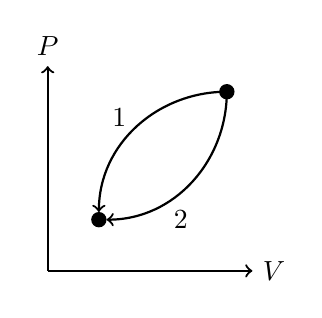
\begin{tikzpicture}[scale=1.3]
        \draw[thick,->](0,0)--(2,0) node[pos=1,right]{$V$};
        \draw[thick,->](0,0)--(0,2) node[pos=1,above]{$P$};
        \fill[black](1.75,1.75) circle(.075); %node[above]{1};
        \fill[black](0.5,0.5) circle(.075); %node[below]{2};
        \draw[thick,->](1.75,1.75) to[out=180,in=90] (.5,.575);
        \draw[thick,->](1.75,1.75) to[out=270,in=0] (.575,.5);
        \node at (1.3,.5) {2}; %[midway,above]{1};
        \node at (.7,1.5) {1}; %[midway,above]{1};
      \end{tikzpicture}
    \end{center}
    \begin{enumerate}[noitemsep,topsep=0pt,leftmargin=18pt,label=(\Alph*)]
    \item $\Delta U_1 = \Delta U_2$ and $W_1= W_2$
    \item $\Delta U_1 = \Delta U_2$ and $W_1>W_2$
    \item $\Delta U_1 > \Delta U_2$ and $W_1=W_2$
    \item $\Delta U_1 > \Delta U_2$ and $W_1\geq W_2$
    \end{enumerate}
  
  \item The figure shows four samples of gas being taken through four
    different processes. Process 1 is adiabatic. In which process is heat being
    transferred to the gas sample from the environment?
    \begin{center}
      \vspace{-.15in}
      \pic{.35}{mc-q22.png}
    \end{center}
    \begin{enumerate}[noitemsep,topsep=0pt,leftmargin=18pt,label=(\Alph*)]
    \item\num{1}
    \item\num{2}
    \item\num{3}
    \item\num{4}
    \end{enumerate}

    \columnbreak
    
  \item Two sealed cylinders holding different gases are placed one on top of
    the other so heat can flow between them. Cylinder A is filled with
    hydrogen. Cylinder B is filled with helium moving with an average speed
    that is half that of the hydrogen atoms. Helium atoms have four times the
    mass of hydrogen atoms. Which of the following best describes the transfer
    of heat between the two containers by conduction?
    \begin{enumerate}[noitemsep,topsep=0pt,leftmargin=18pt,label=(\Alph*)]
    \item Net heat flows from cylinder A to cylinder B, because heat flows from
      higher kinetic energy atoms to lower kinetic energy atoms.
    \item Net heat flows from cylinder B to cylinder A, because heat flows from
      higher kinetic energy atoms to lower kinetic energy atoms.
    \item There is no net heat transfer between the two cylinders, because both
      gases have the same average atomic kinetic energy.
    \item There is no net heat transfer between the two cylinders, because heat
      conduction requires the movement of atoms between the cylinder, and the
      cylinders are sealed.
    \end{enumerate}
  \end{enumerate}

  \columnbreak
  
  \textbf{Questions 24 and 25}

  A gas beginning at point O on the graph can be taken along four paths to
  different ending conditions.
  \begin{center}
    \vspace{-.15in}
    \pic{.35}{mc-q24-25.png}
  \end{center}
  \begin{enumerate}[leftmargin=18pt,start=24]

  \item Which of the following are the same for processes 2 and 3?
    \emph{Select two answers.}
    \begin{enumerate}[noitemsep,topsep=0pt,leftmargin=18pt,label=(\Alph*)]
    \item $Q$
    \item $\Delta T$
    \item $\Delta U$
    \item $W$
    \end{enumerate}
    
  \item Along which of the paths is the most thermal energy removed from the
    gas?
    \begin{enumerate}[noitemsep,topsep=0pt,leftmargin=18pt,label=(\Alph*)]
      \item\num{1}
      \item\num{2}
      \item\num{3}
      \item\num{4}
    \end{enumerate}

    \columnbreak
    
  \item The graph shows the distribution of speeds for one mole of hydrogen at
    temperature $T$, pressure $P$, and volume $V$. How would the graph change
    if the sample was changed from one mole hydrogen to one mole of argon at
    the same temperature, pressure, and volume?
    \begin{center}
      \vspace{-.15in}
      \pic{.35}{mc-q26.png}
    \end{center}
    \begin{enumerate}[noitemsep,topsep=0pt,leftmargin=18pt,label=(\Alph*)]
    \item The peak will shift to the left
    \item The peak will shift upward and to the left
    \item The peak will shift to the right
    \item The peak will shift downward and to the right
    \end{enumerate}
    
  \item The graph shows the pressure and volume of a gas being taken from state
    \#1 to state \#2. Which of the following correctly indicates the sign of
    the work done by the gas, and the change in temperature of the gas?
    \begin{center}
      \vspace{-.15in}
      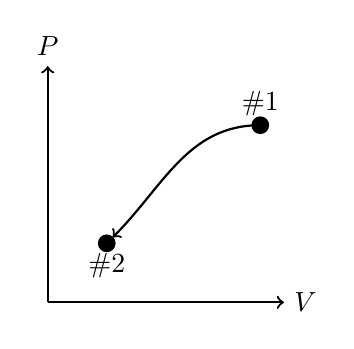
\begin{tikzpicture}[scale=1.5]
        \draw[thick,->](0,0)--(2,0)
        node[pos=1,right]{$V$};
        \draw[thick,->](0,0)--(0,2) node[pos=1,above]{$P$};
        \fill[black](1.8,1.5) circle(.075) node[above]{\#1};
        \fill[black](0.5,0.5) circle(.075) node[below]{\#2};
        \draw[thick,->](1.8,1.5) to[out=180,in=45] (.55,.55);
      \end{tikzpicture}

      \begin{tabular}{ccc}
        & \textbf{Work done} & $\Delta$ \textbf{Temperature}\\ \hline
        (A) & $+$ & $+$ \\
        (B) & $+$ & $-$ \\
        (C) & $-$ & $+$ \\
        (D) & $-$ & $-$
      \end{tabular}
    \end{center}

    \columnbreak
    
  \item A fixed mass of oxygen (O\textsubscript{2}, molecular mass
    \SI{32}{g/mol}) is contained in a cylinder whose volume is \num{2.80}
    liters. The pressure is \SI{148}{atm} when the temperature is
    \SI{23}{\celsius}. Find the mass of oxygen in the cylinder.
    \begin{enumerate}[noitemsep,topsep=0pt,leftmargin=18pt,label=(\Alph*)]
    \item\SI{20}{\gram}
    \item\SI{80}{\gram}
    \item\SI{140}{\gram}
    \item\SI{280}{\gram}
    \item\SI{546}{\gram}
    \end{enumerate}

  \item A tire is filled with air at \SI{15}{\celsius} to a gauge pressure of
    \SI{2.2e5}{\pascal}. If the tire reaches a temperature of \SI{38}{\celsius},
    what will the new gauge pressure be inside it?
    \begin{enumerate}[noitemsep,topsep=0pt,leftmargin=18pt,label=(\Alph*)]
    \item\SI{2.4e2}{\pascal}
    \item\SI{3.4e3}{\pascal}
    \item\SI{2.4e5}{\pascal}
    \item\SI{6.0e7}{\pascal}
    \item\SI{8.0e9}{\pascal}
    \end{enumerate}

  \item A fixed mass of an ideal gas having a volume of \SI{2500}{cm^3} at
    \SI{20}{\celsius} and absolute pressure of \SI{65}{atm} expands until its
    volume is \SI{4000}{cm^3} and its absolute pressure is \SI{45}{atm}. Find
    its new temperature.
    \begin{enumerate}[noitemsep,topsep=0pt,leftmargin=18pt,label=(\Alph*)]
    \item\SI{20}{\celsius}
    \item\SI{42.3}{\celsius}
    \item\SI{51.6}{\celsius}
    \item\SI{61.8}{\celsius}
    \item\SI{80}{\celsius}
    \end{enumerate}

  \item A fixed mass of an ideal gas is in a container with a constant volume.
    By what factor will the pressure change if the absolute temperature is
    tripled?
    \begin{enumerate}[noitemsep,topsep=0pt,leftmargin=18pt,label=(\Alph*)]
    \item 1/9
    \item 1/3
    \item 3
    \item 9
    \end{enumerate}

  \item When using the ideal gas law, $PV=nRT$,
    \begin{enumerate}[noitemsep,topsep=0pt,leftmargin=18pt,label=(\Alph*)]
    \item $P$ can be gauge pressure
    \item $N$ can be in kilograms
    \item $T$ can be in degrees Celsius
    \item none of the above
    \end{enumerate}

    \columnbreak
    
  \item For ideal gases, the ratio $PV/T $ is
    \begin{enumerate}[noitemsep,topsep=0pt,leftmargin=18pt,label=(\Alph*)]
    \item equal to Avogadro's number
    \item equal to Boltzmann's constant
    \item independent of the number of molecules
    \item independent of the chemical nature of the molecules
    \end{enumerate}

  \item The volume of an ideal gas at constant pressure is proportional to its
    \begin{enumerate}[noitemsep,topsep=0pt,leftmargin=18pt,label=(\Alph*)]
    \item Fahrenheit temperature
    \item Celsius temperature
    \item Absolute temperature
    \item Molar mass
    \end{enumerate}

  \item If the pressure of gas is doubled and the temperature is constant, then
    the volume is what factor times the original?
    \begin{enumerate}[noitemsep,topsep=0pt,leftmargin=18pt,label=(\Alph*)]
    \item 2
    \item 1/2
    \item 1/4
    \item 4
    \end{enumerate}

    \columnbreak
    
  \item What is the volume of one mole of ideal gas at \SI{300}{K} and at
    standard atmospheric pressure?
    \begin{enumerate}[noitemsep,topsep=0pt,leftmargin=18pt,label=(\Alph*)]
    \item\SI{23.2}{\litre}
    \item\SI{24.1}{\litre}
    \item\SI{24.6}{\litre}
    \item\SI{25.7}{\litre}
    \end{enumerate}

  \item An ideal gas in a container has a pressure of \SI{2.50}{atm} and a
    volume of \SI{1}{m^3} at a temperature of \SI{30}{\celsius}. How many moles
    of gas are in the container?
    \begin{enumerate}[noitemsep,topsep=0pt,leftmargin=18pt,label=(\Alph*)]
    \item\SI{20}{moles}
    \item\SI{45}{moles}
    \item\SI{62}{moles}
    \item\SI{83}{moles}
    \item\SI{100}{moles}
    \end{enumerate}

  \end{enumerate}
\end{multicols}

%\newpage
%\genanswersheet{2}{Fluid Mechanics \& Thermodynamics}
%
%\begin{center}
%  \begin{minipage}[t]{.2\textwidth}
%    \vspace{.2in}
%    \bgroup
%    \begin{tabular}{>{\centering}m{1.3cm} >{\centering}m{1.7cm}}
%      No. & Answer
%    \end{tabular}\\
%    \def\arraystretch{1.5}
%    \begin{tabular}{|>{\centering}m{1.3cm}|>{\centering}m{1.7cm}|}
%      \hline
%      1 & \\ \hline
%      2 & \\ \hline
%      3 & \\ \hline
%      4 & \\ \hline
%      5 & \\ \hline
%      6 & \\ \hline
%      7 & \\ \hline
%      8 & \\ \hline
%      9 & \\ \hline
%      10 & \\ \hline
%      11 & \\ \hline
%      12 & \\ \hline
%      13 & \\ \hline
%      14 & \\ \hline
%      15 & \\ \hline
%      16 & \\ \hline
%      17 & \\ \hline
%      18 & \\ \hline
%      19 & \\ \hline
%      20 & \\ \hline
%      21 & \\ \hline
%      22 & \\ \hline
%      23 & \\ \hline
%      24 & \\ \hline
%      25 & \\ \hline
%    \end{tabular}
%    \egroup
%  \end{minipage}
%  \hspace{.5in}
%  \begin{minipage}[t]{.2\textwidth}
%    \vspace{.2in}
%    \bgroup
%    \begin{tabular}{>{\centering}m{1.3cm} >{\centering}m{1.7cm}}
%      No. & Answer
%    \end{tabular}\\
%    \def\arraystretch{1.5}
%    \begin{tabular}{|>{\centering}m{1.3cm}|>{\centering}m{1.7cm}|}
%      \hline
%      26 & \\ \hline
%      27 & \\ \hline
%      28 & \\ \hline
%      29 & \\ \hline
%      30 & \\ \hline
%      31 & \\ \hline
%      32 & \\ \hline
%      33 & \\ \hline
%      34 & \\ \hline
%      35 & \\ \hline
%      36 & \\ \hline
%      37 & \\ \hline
%    \end{tabular}
%    \egroup
%  \end{minipage}
%\end{center}
\newpage

\genfreetitle{2}{Fluid Mechanics \& Thermodynamics}{4}

\genfreedirections{15}

\begin{enumerate}[leftmargin=15pt]

\item An air bubble is released from the bottom of a swimming pool and ascends
  to the surface.
  \begin{enumerate}[leftmargin=18pt]
  \item In a clear, coherent, paragraph-length response, describe any
    changes in the bubble size and describe the motion of the bubble
    as it ascends to the surface. Explain the factors that affect the size
    of the bubble and the bubble's motion. Include a description of
    any forces acting on the bubble from the time it is at the bottom of
    the pool until it reaches the surface.
    \vspace{1.75in}
    
  \item Draw a diagram of all the forces acting on the bubble. Make sure
    the forces are in correct proportion.
    \vspace{1.75in}

  \item The bubble does not collapse under the pressure of the water.
    Explain how the behavior of the gas atoms keep the bubble from
    collapsing.
    \newpage
    %\vspace{1.5in}
    
  \item The bubble has an initial volume of $V_D$ , begins at a depth of $D$
    below the surface of the water, and reaches the surface where the
    pressure is $P_S$ . The density of the water is $r$.
    \begin{enumerate}
    \item  Derive an expression for the initial pressure ($P_D$) in the bubble
      in terms of the given quantities and known constants.
    \item Assume the air temperature in the bubble remains the same as
      it rises. Derive an expression for the volume ($V_S$) of the bubble
      when it reaches the surface.
    \end{enumerate}
    \vspace{2in}
    
  \item Now assume that the bubble rises quickly to the surface, and that
    there is negligible thermal energy transfer between the bubble andthe
    swimming pool. Base your answers on this assumption.
    \begin{enumerate}
    \item Sketch the process on the $PV$ diagram. Indicate on the axis the
      initial and final pressures and volumes.
    \item How does the value $P_S$--$V_S$ compare to the value $P_D$--$V_D$?
      %__Greater than P D V D __Equal to P D V D __Less than P D V D
      Justify your answer.
    \end{enumerate}
    \vspace{1.75in}
    
  \item The bubble passes through higher temperature water as it nears the
    sun-warmed surface of the pool. Unexpectedly, this allows a
    sizable amount of thermal energy to transfer from the water to the
    bubble as it rises. How does this affect the final volume of the
    bubble? Justify your answer.
  \end{enumerate}
  \newpage
  
\item A \SI{1.0}{cm} radius hose with a \SI{0.50}{cm} radius exit nozzle is
  being used to fill a \SI{1000}{ml} beaker with oil\\
  (\SI{1000}{ml}=\SI{0.0010}{m^3}). The velocity of the oil in the hose is
  $v=\SI{0.40}{m/s}$ as shown in the figure. The density of the oil is
  \SI{960}{kg/m^3}, and the atmospheric pressure is \SI{1.01e5}{\pascal}.
  \begin{center}
    \pic{.38}{fr-q2.png}
  \end{center}
  
  \begin{enumerate}[leftmargin=18pt]
  \item The nozzle attached to the end of the hose has a smaller radius
    than the hose. If the nozzle is removed from the hose, will the
    beaker be filled faster? Justify your answer with conservation
    laws.
    \vspace{.75in}
    
  \item Calculate the exit velocity of the oil from the nozzle.
    \vspace{.75in}
    
  \item How long will it take to fill the beaker?
    \vspace{.75in}
    
  \item Point A is shown in the figure. How does the pressure in the fluid
    at point A compare to the pressure in the fluid at the exit nozzle?
    Justify your claim.
    \vspace{.75in}
    
  \item The hose is now used to fill a \SI{200}{\milli\litre} graduated
    cylinder with oil to the same height as the height of the oil in the
    \SI{1000}{\milli\litre} beaker. Compare the net force from the oil on the
    bottom of the \SI{200}{\milli\litre} cylinder and the
    \SI{1000}{\milli\litre}. Explain your answer.
    \vspace{1in}
    
  \item A cube of lead with a side dimension of \SI{5.0}{cm} is slowly lowered
    into the beaker of oil by a thin string attached to a spring scale at a
    constant rate, as shown in the figure. The density of lead is
    \SI{11300}{kg/m^3}.
    \begin{center}
      \pic{.3}{fr-2a.png}
    \end{center}
    \begin{enumerate}
    \item What will be the spring scale reading in newtons when the lead has
      been submerged to location 2?
    \item Does the spring scale reading increase, decrease, or stay the
      same when the cube is lowered from location 2 to location 3?
      Justify your answer by referencing the pressure of the fluid on
      the lead cube.
    \item The lead cube is lowered from above the oil’s surface (location
      1) to a spot just below the surface (location 2) until the cube is
      just above the bottom of the beaker (location 3). Describe any
      changes in pressure on the bottom of the beaker during this
      process. Explain your answer.
    \end{enumerate}
  \end{enumerate}
  \newpage
  
\item A mole of ideal gas is enclosed in a cylinder with a movable piston
  with a cross-sectional area of \SI{1e-2}{m^2}. The gas is taken through a
  thermodynamic process, as shown in the figure.
  \begin{center}
    \pic{.4}{fr-q3a.png}
  \end{center}
  \begin{enumerate}[leftmargin=18pt]
  \item Calculate the temperature of the gas at state A, and describe the
    microscopic property of the gas that is related to the
    temperature.
    \vspace{1in}
  \item Calculate the force of the gas on the piston at state A, and
    explain how the atoms of the gas exert this force on the piston.
    \vspace{1in}
  \item Predict qualitatively the change in the internal energy of the gas
    as it is taken from state B to state C. Justify your prediction.
    \vspace{1in}
  \item Is heat transferred to or from the gas as it is taken from state B to
    state C? Justify your answer.
    \newpage

  \item Discuss any entropy changes in the gas as it is taken from state B
    to state C. Justify your answer.
    \vspace{1in}
  \item Calculate the change in the total kinetic energy of the gas atoms
    as the gas is taken from state C to state A.
    \vspace{1in}
  \item On the axis provided, sketch and label the distribution of the speeds
    of the atoms in the gas for states A and B.
    \begin{center}
      \begin{tikzpicture}[scale=4]
        \draw[very thick,->](0,0)--(3,0)
        node[midway,below]{speed};
        \draw[very thick,->](0,0)--(0,2)
        node[midway,above,sloped]{number of atoms};
      \end{tikzpicture}
    \end{center}
  \end{enumerate}

\item You wish to determine the relationship between gas pressure and
  temperature.
  \begin{enumerate}[leftmargin=18pt]
  \item List the items you would use to perform this investigation.
    \newpage
    
  \item Draw a simple picture of the lab setup, and outline the experimental
    procedure you would use to gather the necessary data. Indicate the
    measurements to be taken and how the measurement will be used to obtain the
    data needed. Make sure your outline contains sufficient detail so that
    another student could follow your procedure.
    \vspace{1.75in}
  \item On the axis, sketch the line or curve that you predict will represent
    the results of the data gathered in this experiment.
    \begin{center}
      \begin{tikzpicture}[scale=1.75]
        \draw[very thick,->](0,0)--(2,0) node[pos=1,right]{$P$};
        \draw[very thick,->](0,0)--(0,2) node[pos=1,above]{$T$};
      \end{tikzpicture}
    \end{center}
    
  \item Explain how you could use your results to estimate the value of
    absolute zero.
  \end{enumerate}

  You are given the following set of data acquired in a gas laboratory
  experiment and asked to determine the relationship between pressures and
  volume for the gas.
  \begin{center}
    \vspace{-.1in}
    \pic{.39}{fr-q4.png}
  \end{center}
  \begin{enumerate}[start=5]
  \item Which subset of the data would be most useful in creating a graph to
    determine the relationship between gas pressure and volume? Explain why the
    trials you selected are the most useful.
    \vspace{1.25in}
    
  \item Plot the subset of data you chose on the graph, being sure to label the
    axes. Draw a line or curve that best represents the relationship between
    the variables.
    \begin{center}
      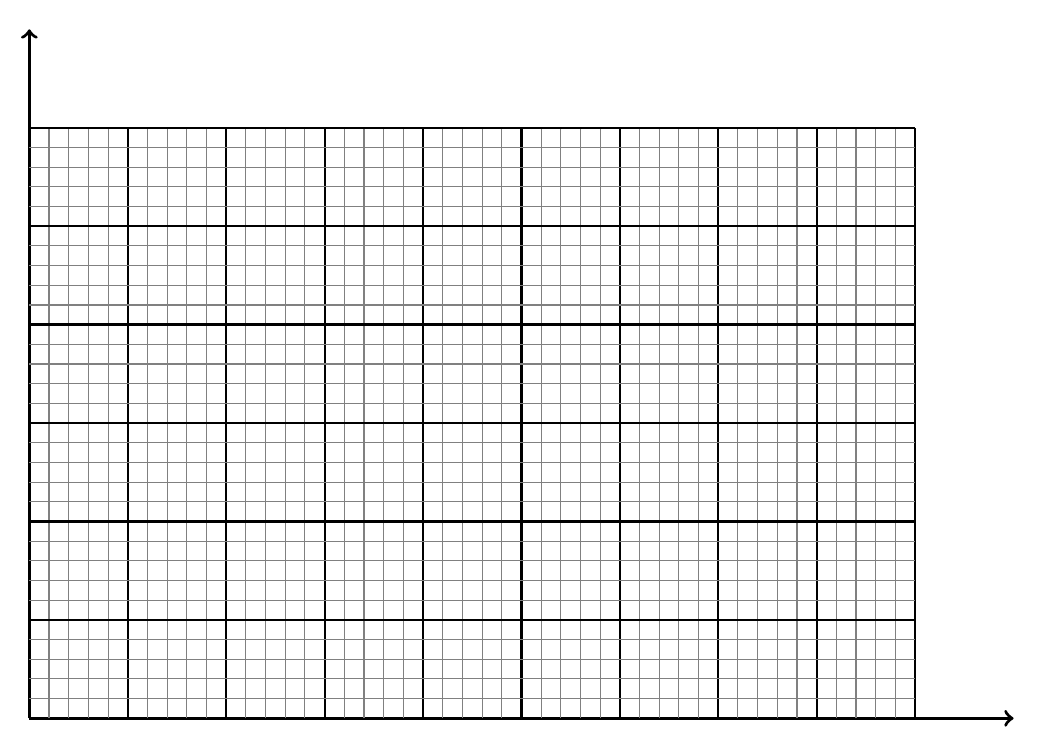
\begin{tikzpicture}[scale=2.5]
        \draw[very thick,->](0,0)--(5,0);
        \draw[very thick,->](0,0)--(0,3.5);
        \foreach \x in {.1,.2,...,4.5} \draw[gray](\x,0)--(\x,3);
        \foreach \xx in {.5,1,...,4.5} \draw[thick](\xx,0)--(\xx,3);
        \foreach \y in {.1,.2,...,3}   \draw[gray](0,\y)--(4.5,\y);
        \foreach \yy in {.5,1,...,3}   \draw[thick](0,\yy)--(4.5,\yy);
      \end{tikzpicture}
    \end{center}
  \item What can you conclude from your line or curve about the relationship
    between volume and pressure?
  \end{enumerate}
\end{enumerate}
\end{document}
